\documentclass[8pt,aspectratio=169]{beamer}
\usetheme{Madrid}
\usepackage{graphicx}
\usepackage{booktabs}
\usepackage{adjustbox}
\usepackage{multicol}
\usepackage{amsmath}
\usepackage{amssymb}
\usepackage{tikz}
\usetikzlibrary{arrows.meta,positioning,shapes.callouts,shapes.geometric,decorations.pathreplacing}
\usepackage{colortbl}
\usepackage{pgfplots}
\pgfplotsset{compat=1.18}
\usepackage{hyperref}
\usepackage{algorithm}
\usepackage{algorithmic}

% Color definitions
\definecolor{mlblue}{RGB}{0,102,204}
\definecolor{mlpurple}{RGB}{51,51,178}
\definecolor{mllavender}{RGB}{173,173,224}
\definecolor{mllavender2}{RGB}{193,193,232}
\definecolor{mllavender3}{RGB}{204,204,235}
\definecolor{mllavender4}{RGB}{214,214,239}
\definecolor{mlorange}{RGB}{255, 127, 14}
\definecolor{mlgreen}{RGB}{44, 160, 44}
\definecolor{mlred}{RGB}{214, 39, 40}
\definecolor{mlgray}{RGB}{127, 127, 127}

% Additional colors for template compatibility
\definecolor{lightgray}{RGB}{240, 240, 240}
\definecolor{midgray}{RGB}{180, 180, 180}
\definecolor{dfteal}{RGB}{0,128,128}
\definecolor{dfred}{RGB}{180,30,30}

% Backward compatibility: uppercase color names
\colorlet{MLPurple}{mlpurple}
\colorlet{MLBlue}{mlblue}
\colorlet{MLOrange}{mlorange}
\colorlet{MLGreen}{mlgreen}
\colorlet{MLRed}{mlred}
\colorlet{MLLavender}{mllavender}
\colorlet{MLGray}{mlgray}

% Apply custom colors to Madrid theme
\setbeamercolor{palette primary}{bg=mllavender3,fg=mlpurple}
\setbeamercolor{palette secondary}{bg=mllavender2,fg=mlpurple}
\setbeamercolor{palette tertiary}{bg=mllavender,fg=white}
\setbeamercolor{palette quaternary}{bg=mlpurple,fg=white}

\setbeamercolor{structure}{fg=mlpurple}
\setbeamercolor{section in toc}{fg=mlpurple}
\setbeamercolor{subsection in toc}{fg=mlblue}
\setbeamercolor{title}{fg=mlpurple}
\setbeamercolor{frametitle}{fg=mlpurple,bg=mllavender3}
\setbeamercolor{block title}{bg=mllavender2,fg=mlpurple}
\setbeamercolor{block body}{bg=mllavender4,fg=black}

% Remove navigation symbols
\setbeamertemplate{navigation symbols}{}

% Clean itemize/enumerate
\setbeamertemplate{itemize items}[circle]
\setbeamertemplate{enumerate items}[default]

% Reduce margins for more content space
\setbeamersize{text margin left=5mm,text margin right=5mm}

% Custom course footer
\setbeamertemplate{footline}{
  \leavevmode%
  \hbox{%
    \begin{beamercolorbox}[wd=.333333\paperwidth,ht=2.25ex,dp=1ex,center]{author in head/foot}%
      \usebeamerfont{author in head/foot}Methods and Algorithms
    \end{beamercolorbox}%
    \begin{beamercolorbox}[wd=.333333\paperwidth,ht=2.25ex,dp=1ex,center]{title in head/foot}%
      \usebeamerfont{title in head/foot}MSc Data Science
    \end{beamercolorbox}%
    \begin{beamercolorbox}[wd=.333333\paperwidth,ht=2.25ex,dp=1ex,right]{date in head/foot}%
      \usebeamerfont{date in head/foot}\insertframenumber{} / \inserttotalframenumber\hspace*{2ex}
    \end{beamercolorbox}}%
  \vskip0pt%
}

% Command for bottom annotation (Madrid-style)
\newcommand{\bottomnote}[1]{%
\vfill
\vspace{-2mm}
\textcolor{mllavender2}{\rule{\textwidth}{0.4pt}}
\vspace{1mm}
\footnotesize
\textbf{#1}
}

% Custom commands for course compatibility
\newcommand{\highlight}[1]{\textcolor{mlorange}{\textbf{#1}}}
\newcommand{\mathbold}[1]{\boldsymbol{#1}}

% Compact list environment
\newenvironment{compactlist}{%
  \begin{itemize}%
    \setlength{\itemsep}{2pt}%
    \setlength{\parskip}{0pt}%
    \setlength{\parsep}{0pt}%
}{%
  \end{itemize}%
}

\title[L06e: Modern RL]{Modern Reinforcement Learning: A Practical Guide}
\subtitle{How to Use RL in 2025 with Gymnasium, PPO, and RLHF}
\author{Prof.\ Dr.\ J\"org Osterrieder}
\institute{Methods and Algorithms --- MSc Data Science}
\date{Spring 2026}

\begin{document}

% Slide 1: Title Page
\begin{frame}[plain]
\titlepage
\end{frame}

% Slide 2: TikZ Opening Comic
\begin{frame}{You Know RL --- Now How Do People Actually Use It?}
\begin{columns}[c]
\begin{column}{0.40\textwidth}
\centering
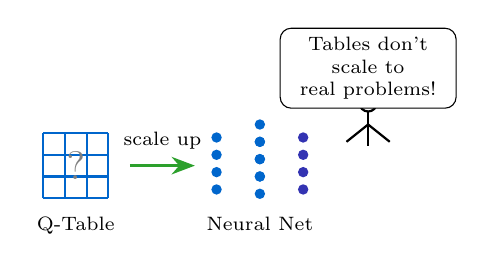
\begin{tikzpicture}[scale=0.55]
  % Small Q-table (left side)
  \draw[step=0.5, mlblue, thick] (0,0) grid (1.5,1.5);
  \node[font=\scriptsize, below] at (0.75,-0.2) {Q-Table};
  \node[font=\Large, mlgray] at (0.75,0.75) {?};
  % Arrow
  \draw[-{Stealth}, very thick, mlgreen] (2.0,0.75) -- (3.5,0.75);
  \node[font=\scriptsize, above] at (2.75,0.9) {scale up};
  % Neural network (right side)
  \foreach \y in {0.2,0.6,1.0,1.4} {
    \fill[mlblue] (4.0,\y) circle (0.12);
    \fill[mlblue] (5.0,\y-0.1) circle (0.12);
    \fill[mlblue] (5.0,\y+0.3) circle (0.12);
    \fill[mlpurple] (6.0,\y) circle (0.12);
  }
  \node[font=\scriptsize, below] at (5.0,-0.2) {Neural Net};
  % Stick figure with speech bubble
  \draw[thick] (7.5,2.2) circle (0.2);
  \draw[thick] (7.5,2.0) -- (7.5,1.2);
  \draw[thick] (7.5,1.7) -- (7.0,1.3);
  \draw[thick] (7.5,1.7) -- (8.0,1.3);
  \node[draw, rounded corners, fill=white, font=\scriptsize, text width=2cm, align=center] at (7.5,3.0) {Tables don't\\scale to\\real problems!};
\end{tikzpicture}
\end{column}
\begin{column}{0.55\textwidth}
\large
\textit{You already know what RL is (L06b). Now: how do practitioners actually \textbf{use} it today?}

\vspace{5mm}
\begin{compactlist}
\item Deep RL libraries that work out of the box
\item PPO as the workhorse algorithm
\item RLHF --- how ChatGPT learned to be helpful
\end{compactlist}
\end{column}
\end{columns}
\bottomnote{From Q-tables to neural networks: modern RL scales to any problem.}
\end{frame}

% Slide 3: TikZ Comic C1 --- "The Scale Problem"
\begin{frame}{The Scale Problem: Why Tables Break Down}
\centering
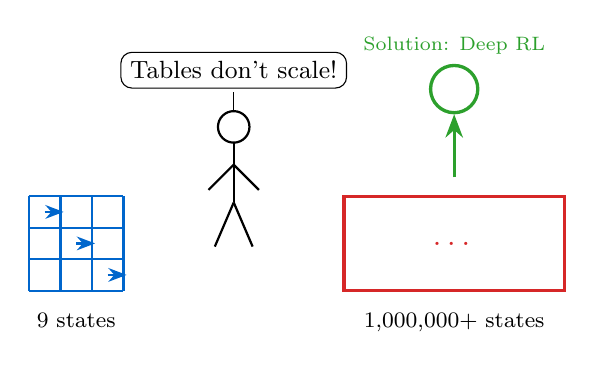
\begin{tikzpicture}[scale=0.8]
% Small grid (left)
\draw[step=0.5, mlblue, thick] (0,0) grid (1.5,1.5);
\foreach \x/\y in {0.25/1.25, 0.75/0.75, 1.25/0.25} {
  \draw[-{Stealth}, mlblue, thick] (\x,\y) -- ++(0.3,0);
}
\node[font=\footnotesize, below] at (0.75,-0.2) {9 states};
% Large block (right)
\draw[mlred, very thick] (5,0) rectangle (8.5,1.5);
\node[font=\large, mlred] at (6.75,0.75) {\ldots};
\node[font=\footnotesize, below] at (6.75,-0.2) {1,000,000+ states};
% Stick figure (middle)
\draw[thick] (3.25,2.6) circle (0.25);
\draw[thick] (3.25,2.35) -- (3.25,1.4);
\draw[thick] (3.25,2.0) -- (2.85,1.6);
\draw[thick] (3.25,2.0) -- (3.65,1.6);
\draw[thick] (3.25,1.4) -- (2.95,0.7);
\draw[thick] (3.25,1.4) -- (3.55,0.7);
% Speech bubble
\node[draw, rounded corners, fill=white, font=\small] at (3.25,3.5) {Tables don't scale!};
\draw (3.25,3.15) -- (3.25,2.85);
% Arrow to neural net icon
\draw[-{Stealth}, very thick, mlgreen] (6.75,1.8) -- (6.75,2.8);
\node[circle, draw=mlgreen, very thick, minimum size=6mm] at (6.75,3.2) {};
\node[font=\scriptsize, mlgreen, above] at (6.75,3.6) {Solution: Deep RL};
\end{tikzpicture}

\vspace{3mm}
Classic RL stores a table of values. Modern RL uses neural networks to handle any state space.
\bottomnote{A chess board has $\sim$10$^{44}$ possible states. No table can store that. Neural networks generalize.}
\end{frame}

% Slide 4: From Tables to Neural Networks
\begin{frame}{From Tables to Neural Networks}
\begin{columns}[T]
\begin{column}{0.47\textwidth}
\textcolor{mlred}{\textbf{Classic RL (L06b)}}
\begin{compactlist}
\item Q-table stores one value per state
\item Works for small grids (9--100 states)
\item Tabular lookup --- no generalization
\end{compactlist}
\end{column}
\begin{column}{0.47\textwidth}
\textcolor{mlgreen}{\textbf{Modern RL (Today)}}
\begin{compactlist}
\item Neural network approximates Q-values
\item Works for any state space (millions+)
\item Learns to generalize across states
\end{compactlist}
\end{column}
\end{columns}

\vspace{4mm}
\begin{block}{The Key Insight}
Replace the table with a neural network = Deep RL.
\end{block}
\bottomnote{DQN (2015) was the breakthrough: a neural network that plays Atari games from raw pixels.}
\end{frame}

% Slide 5: CHART --- DQN Architecture
\begin{frame}{DQN: The Neural Network That Plays Atari}
\centering

\includegraphics[width=0.60\textwidth]{09_dqn_architecture/chart.pdf}
\begin{compactlist}
\item State (pixels, numbers) goes into the neural network
\item Network outputs a Q-value for every possible action
\item Pick the action with the highest Q-value
\end{compactlist}
\bottomnote{DQN = Deep Q-Network. DeepMind used this to beat human experts at 49 Atari games (2015).}
\end{frame}

% Slide 6: The Modern RL Stack
\begin{frame}{The Modern RL Stack}
\centering
\small
\begin{tabular}{l l}
\toprule
\textbf{Layer} & \textbf{Tool} \\
\midrule
Environments & Gymnasium (successor to OpenAI Gym) \\
Algorithms & Stable-Baselines3 (PPO, SAC, DQN pre-built) \\
Training & GPU-accelerated (thousands of episodes/second) \\
Monitoring & Weights \& Biases, TensorBoard \\
Deployment & ONNX export, sim-to-real transfer \\
\bottomrule
\end{tabular}

\vspace{4mm}
\highlight{Everything you need is open-source and pip-installable.}
\bottomnote{pip install gymnasium stable-baselines3. That is all you need to start training RL agents today.}
\end{frame}

% Slide 7: CHART --- PPO Training Curve (NEW)
\begin{frame}{PPO: The Workhorse Algorithm}
\centering

\includegraphics[width=0.65\textwidth]{15_ppo_training_curve/chart.pdf}
\begin{compactlist}
\item PPO learns fast: solves CartPole in \raise.17ex\hbox{$\scriptstyle\sim$}30k timesteps
\item Stable updates: no catastrophic performance drops
\item The default choice for most RL tasks in 2025
\end{compactlist}
\bottomnote{PPO = Proximal Policy Optimization (Schulman et al., 2017). Used by OpenAI, DeepMind, and most practitioners.}
\end{frame}

% Slide 8: RLHF --- How ChatGPT Learned to Be Helpful
\begin{frame}{RLHF --- How ChatGPT Learned to Be Helpful}
\begin{enumerate}
\setlength{\itemsep}{6pt}
\item \textbf{Train a base LLM} on text data (supervised learning)
\item \textbf{Humans rank outputs} --- which response is better?
\item \textbf{RL (PPO!) fine-tunes} the LLM to match human preferences
\end{enumerate}

\vspace{3mm}
\begin{block}{RLHF = Reinforcement Learning from Human Feedback}
The reward signal comes from human preferences, not a score function.
\end{block}

\vspace{2mm}
\highlight{The same PPO from Slide 7 is used to align ChatGPT.}
\bottomnote{InstructGPT paper (Ouyang et al., 2022) introduced RLHF for language models. Now standard for all frontier LLMs.}
\end{frame}

% Slide 8b: RLHF Pipeline Diagram
\begin{frame}{What Does the RLHF Pipeline Look Like?}
\centering

\includegraphics[width=0.65\textwidth]{18_rlhf_pipeline/chart.pdf}
\begin{compactlist}
\item Three stages: supervised learning, then human feedback, then PPO
\item The reward model learns what humans prefer
\item PPO optimizes the LLM to maximize the learned reward
\end{compactlist}
\bottomnote{This exact 3-stage pipeline is used by OpenAI (ChatGPT), Anthropic (Claude), and Google (Gemini).}
\end{frame}

% Slide NEW: Offline RL
\begin{frame}{What If You Can't Explore? Offline RL}
\begin{columns}[c]
\begin{column}{0.50\textwidth}
\centering

\includegraphics[width=\textwidth]{23_offline_vs_online_rl/chart.pdf}
\end{column}
\begin{column}{0.45\textwidth}
\begin{compactlist}
\item \textbf{Online RL}: agent explores freely (games, robotics)
\item \textbf{Offline RL}: learn from a fixed dataset --- no new interaction
\item Finance: live trading exploration is expensive and risky
\item Key methods: CQL (Conservative Q-Learning), Decision Transformer
\end{compactlist}
\vspace{3mm}
\highlight{Offline RL is the most finance-relevant RL frontier.}
\end{column}
\end{columns}
\bottomnote{Offline RL learns from historical data only --- critical when online exploration is too costly or dangerous.}
\end{frame}

% Slide NEW: FinRL Framework
\begin{frame}{FinRL: A Ready-Made Framework for Financial RL}
\vspace{2mm}
\footnotesize
\texttt{from finrl.agents.stablebaselines3 import DRLAgent}\\[2pt]
\texttt{from finrl.meta.env\_stock\_trading import StockTradingEnv}\\[4pt]
\texttt{env = StockTradingEnv(df=stock\_data)}\\[2pt]
\texttt{agent = DRLAgent(env)}\\[2pt]
\texttt{model = agent.get\_model("ppo")}\\[2pt]
\texttt{trained = agent.train\_model(model, total\_timesteps=50000)}

\vspace{5mm}
\normalsize
\begin{compactlist}
\item Pre-built trading environments (stocks, crypto, portfolio)
\item Handles data download, feature engineering, backtesting
\item Supports PPO, A2C, DDPG, SAC out of the box
\end{compactlist}
\bottomnote{FinRL: github.com/AI4Finance-Foundation/FinRL (Liu et al., 2021). pip install finrl.}
\end{frame}

% Slide 9: Sim-to-Real + Applications
\begin{frame}{Where Modern RL Shines}
\begin{columns}[c]
\begin{column}{0.50\textwidth}
\centering

\includegraphics[width=\textwidth]{13_walkforward_timeline/chart.pdf}
\end{column}
\begin{column}{0.45\textwidth}
\begin{compactlist}
\item \textbf{Game AI}: AlphaGo, OpenAI Five
\item \textbf{Robotics}: sim-to-real transfer
\item \textbf{Finance}: walk-forward validated trading
\end{compactlist}

\vspace{3mm}
Train millions of episodes in simulation (free, fast, safe), then deploy.
\end{column}
\end{columns}
\bottomnote{Sim-to-real: train in simulation where mistakes are free, then fine-tune on real data.}
\end{frame}

% Slide 10: Try It Yourself --- Five Lines of Python
\begin{frame}{Try It Yourself --- Five Lines of Python}
\vspace{2mm}
\footnotesize
\texttt{from stable\_baselines3 import PPO}\\[2pt]
\texttt{import gymnasium as gym}\\[4pt]
\texttt{env = gym.make("CartPole-v1")}\\[2pt]
\texttt{model = PPO("MlpPolicy", env)}\\[2pt]
\texttt{model.learn(total\_timesteps=50\_000)}

\vspace{5mm}
\normalsize
\highlight{Five lines. That is a complete RL training pipeline.}
\bottomnote{pip install stable-baselines3[extra]. CartPole is the ``Hello World'' of RL. Try LunarLander-v3 next!}
\end{frame}

% Slide 11: TikZ Comic C2 + XKCD Closing
\begin{frame}{Key Takeaways}
\begin{columns}[c]
\begin{column}{0.35\textwidth}
\centering
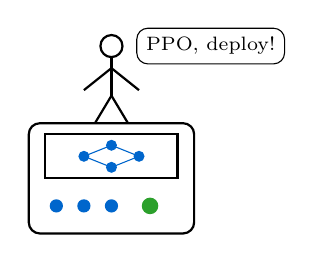
\begin{tikzpicture}[scale=0.7]
% Control panel
\draw[thick, rounded corners] (0,0) rectangle (3,2);
\foreach \x in {0.5,1.0,1.5} {\fill[mlblue] (\x,0.5) circle (0.12);}
\fill[mlgreen] (2.2,0.5) circle (0.15);
% Screen with neural net icon
\draw[thick] (0.3,1.0) rectangle (2.7,1.8);
\fill[mlblue] (1.0,1.4) circle (0.1);
\fill[mlblue] (1.5,1.2) circle (0.1);
\fill[mlblue] (1.5,1.6) circle (0.1);
\fill[mlblue] (2.0,1.4) circle (0.1);
\draw[mlblue] (1.0,1.4) -- (1.5,1.2);
\draw[mlblue] (1.0,1.4) -- (1.5,1.6);
\draw[mlblue] (1.5,1.2) -- (2.0,1.4);
\draw[mlblue] (1.5,1.6) -- (2.0,1.4);
% Stick figure
\draw[thick] (1.5,3.4) circle (0.2);
\draw[thick] (1.5,3.2) -- (1.5,2.5);
\draw[thick] (1.5,3.0) -- (1.0,2.6);
\draw[thick] (1.5,3.0) -- (2.0,2.6);
\draw[thick] (1.5,2.5) -- (1.2,2.0);
\draw[thick] (1.5,2.5) -- (1.8,2.0);
% Speech bubble
\node[draw, rounded corners, fill=white, font=\scriptsize] at (3.3,3.4) {PPO, deploy!};
\end{tikzpicture}
\end{column}
\begin{column}{0.60\textwidth}
\begin{enumerate}
\setlength{\itemsep}{5pt}
\item Modern RL uses neural networks, not tables (Deep RL)
\item PPO is the workhorse algorithm; RLHF uses it to align LLMs
\item Gymnasium + Stable-Baselines3 = 5 lines to a trained agent
\end{enumerate}
\end{column}
\end{columns}
\bottomnote{Next: try the RL notebook to train your own PPO agent!}
\end{frame}

\end{document}
